% ==============================================================================
% TCC - Nome do Aluno
% Capítulo 2 - Revisão da Literatura
% ==============================================================================
\chapter{Revisão da Literatura}
\label{sec-literatura}

Neste capítulo é feita uma revisão dos principais conceitos utilizados neste
trabalho, além de apresentar fundamentos para uma compreensão mais profunda dos
mesmos.

\section{Redes Neurais Feedfoward}

O primeiro conceito a ser compreender são as redes neurais \textit{feedfoward},
também conhecidas como \textit{perceptrons} de multiplas camadas, do inglês,
\textit{multitayer perceptrons} (\textit{MLP}). Redes \textit{feedfoward} 
podem ser entendidos como um modelo que simula o funcionamento de um cerebro,
em que os neurõnios formam um rede de conexões, em que o processamento se dá
pela passagem de informação por essa rede considerando a topologia, ou seja, as
conexões sinápticas entre os neurõnios e força des mesmas. Sendo que a força
pode ser de ativação (positiva), ou de inibição (negativa).
Nesta analogia, um neurõnio é entendido como uma unidade de processamento que 
ao receber estimulos de outros neurõnios, processa estas entradas e 
produz uma saída. Esta estrutura de neurõnio artificial foi proposta em 
\cite{mcculloch-pitts:1943-perceptron} e está esquematizada na figura 
\ref{fig:neuronio-de-pitts}.  

\begin{figure}[htpb]
\centering
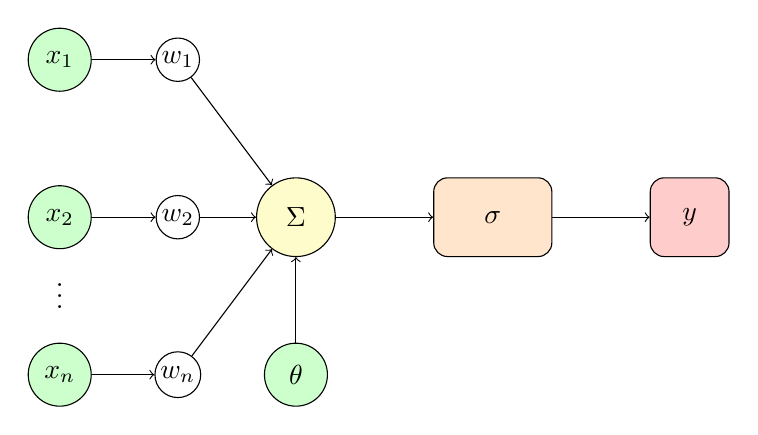
\begin{tikzpicture}[
    neuron/.style={circle, draw=black, fill=blue!20, minimum size=1.2cm},
    input/.style={circle, draw=black, fill=green!20, minimum size=0.8cm},
    weight/.style={fill=white, circle, draw=black, inner sep=1pt},
    arrow/.style={-Stealth, semithick},
    label/.style={text width=2cm, align=center, font=\small\sffamily}
]

\node[input] (x1) at (-3, 2) {$x_1$};
\node[input] (x2) at (-3, 0) {$x_2$};
\node at (-3, -0.9) {$\vdots$};
\node[input] (xn) at (-3, -2) {$x_n$};

\node[weight] (w1) at (-1.5, 2) {$w_1$};
\node[weight] (w2) at (-1.5, 0) {$w_2$};
\node[weight] (wn) at (-1.5, -2) {$w_n$};

\node[draw, circle, minimum size=1cm, fill=yellow!20] (sum) at (0, 0) {$\Sigma$};
\node[draw, rectangle, rounded corners=5pt, minimum width=1.5cm, minimum height=1cm, fill=orange!20] (act) at (2.5, 0) {$\sigma$};
\node[draw, rectangle, rounded corners=5pt, minimum width=1cm, minimum height=1cm, fill=red!20] (out) at (5, 0) {$y$};
\node[input] (b) at (0, -2) {$\theta$};

\draw (x1) edge[->] (w1);
\draw (x2) edge[->] (w2);
\draw (xn) edge[->] (wn);

\draw (w1) edge[->] (sum);
\draw (w2) edge[->] (sum);
\draw (wn) edge[->] (sum);

\draw (b) edge[->] (sum);
\draw (sum) edge[->] (act);
\draw (act) edge[->] (out);

\end{tikzpicture}
\caption{Representação gráfica de um neurónio de MacCough-Pitts. Fonte: elaborada pelos autores.}
\label{fig:neuronio-de-pitts}
\end{figure}

Formalizando matemáticamente a figura \ref{fig:neuronio-de-pitts},
sendo $W$ um vetor de pesos $\in [-1, 1]$, $\boldsymbol{x}$ um vetor de entradas
de tamanho $n$ e pertecente a $R^n$, $\theta$ um valor pertecente a $R$ 
e $\sigma$ uma função não linear. Um neurõnio é uma função $f: R^n \rightarrow R$,

\begin{eqnarray}\label{eq:neuronio-pitts}
    \sigma((\sum_{i=1}^{n} W_i\boldsymbol{x_i}) + \theta)
\end{eqnarray}

O termo $\theta$ pode ser entendido como o último elemento de $\boldsymbol{x}$ 
que está sendo sempre multiplicado pelo último elemento de $W$
que sempre tem valor igual a $1$, logo a equação \ref{eq:neuronio-pitts}
pode ser simplicada como,

\begin{eqnarray}\label{eq:neuronio-pitts-simplificado}
    \sigma(W\boldsymbol{x})
\end{eqnarray}

Um neurõnio pode ser entendido como uma transformação linear, a multiplicação
das entradas pelos pesos e viéses somados, seguida por uma
transformação não linear. Esta é feita pela função de ativação $\sigma$.
Alguns exemplos de funções de ativação empregradas nas redes neurais são A
função \textit{sigmoid} \ref{eq:sigmoid}, 
tangente hiperbólica (\textit{tanh}) \ref{eq:tanh}e 
\textit{Rectfied Linear Unit} (\textit{ReLU}) \ref{eq:relu}.

\begin{eqnarray}
    \text{sigmoid}(x) &=& \frac{e^x}{1 + e^x}\label{eq:sigmoid}
    \\
    \text{tanh}(x) &=& \frac{e^x - e^{-x}}{e^x + e^{-x}}\label{eq:tanh}
    \\ 
    \text{ReLU}(x) &=& \begin{cases} 
                        x & \text{if } x > 0 \\
                        0 & \text{if } x \leq 0 
                    \end{cases}\label{eq:relu}
\end{eqnarray}

Um único neurõnio não é capaz de aproximar qualquer função, para isso, eles são 
organizados em camadas que a saída de cada neurõnio de uma camada forma 
parte da entrada de todos os neurõnios da camada seguinte. 
A primeira camada apenas representa os dados de entrada, a última camada
representa um vetor de saída de tamanho 
Logo, uma rede neural \textit{feedfoward} com $L$ camadas escondidas 
pode ser entendida como uma função composta $f$ formada por 
um conjunto de consecutivas transformações lineares e não lineares num 
vetor de dados de entrada de tamanho $n$ $\boldsymbol{x} \in R^n$
que produz como saída um vetor de tamanho $m$ $\boldsymbol{\hat{y}} \in R^m$,  
sendo as transformações intermediárias representadas pelas saídas $y^l$ 
da camada escondida $l$, $l \in [1,..,L]$,

\begin{equation}\label{eq:rede-neural-composta}
    f(\boldsymbol{x}) = \sigma^{L + 1} y^{L + 1} \circ \sigma^{L} \circ y^{L} 
    \dots \circ \sigma^{2} \circ y^{2} \circ \sigma^{1} \circ y^{1}
\end{equation}

A figura \ref{fig:feedfoward-representacao-grafica} resume graficamente a
definição presente na equação \ref{eq:rede-neural-composta}.

\begin{figure}[htpb]
\centering
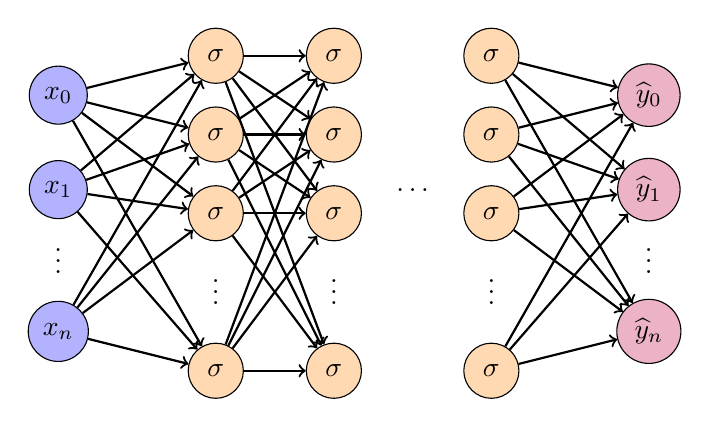
\begin{tikzpicture}[
    neuron/.style={circle, draw, minimum size=0.7cm},
    layer/.style={rectangle, minimum width=1.5cm, minimum height=8cm, draw=black, fill=blue!10, rounded corners=3pt},
    input/.style={neuron, fill=blue!30},
    hidden/.style={neuron, fill=orange!30},
    output/.style={neuron, fill=purple!30},
    physnode/.style={rectangle, draw, rounded corners, fill=orange!30, minimum width=1.5cm, minimum height=1.8cm},
    lossnode/.style={rectangle, draw, rounded corners, fill=yellow!30, minimum width=2cm, minimum height=3.2cm, align=center},
    every edge/.style={draw, ->, thick}
]

\node[input] (I-1) at (0, 3.5) {$x_0$};
\node[input] (I-2) at (0, 2.3) {$x_1$};
\node at (0, 1.5) {$\vdots$};
\node[input] (I-3) at (0, 0.5) {$x_n$};

\node[hidden] (H1-1) at (2, 4) {$\sigma$};
\node[hidden] (H1-2) at (2, 3) {$\sigma$};
\node[hidden] (H1-3) at (2, 2) {$\sigma$};
\node at (2, 1.1) {$\vdots$};
\node[hidden] (H1-4) at (2, 0) {$\sigma$};

\node[hidden] (H2-1) at (3.5, 4) {$\sigma$};
\node[hidden] (H2-2) at (3.5, 3) {$\sigma$};
\node[hidden] (H2-3) at (3.5, 2) {$\sigma$};
\node at (3.5, 1.1) {$\vdots$};
\node[hidden] (H2-4) at (3.5, 0) {$\sigma$};

\node at (4.5, 2.3) {$\dots$};

\node[hidden] (Hn-1) at (5.5, 4) {$\sigma$};
\node[hidden] (Hn-2) at (5.5, 3) {$\sigma$};
\node[hidden] (Hn-3) at (5.5, 2) {$\sigma$};
\node at (5.5, 1.1) {$\vdots$};
\node[hidden] (Hn-4) at (5.5, 0) {$\sigma$};

\node[output] (O-1) at (7.5, 3.5) {$\widehat{y}_0$};
\node[output] (O-2) at (7.5, 2.3) {$\widehat{y}_1$};
\node at (7.5, 1.5) {$\vdots$};
\node[output] (O-3) at (7.5, 0.5) {$\widehat{y}_n$};

% Connections
\foreach \i in {1,2,3}
    \foreach \j in {1,...,4}
        \path (I-\i) edge (H1-\j);

\foreach \i in {1,...,4}
    \foreach \j in {1,...,4}
        \path (H1-\i) edge (H2-\j);

\foreach \i in {1,...,4}
    \foreach \j in {1,...,3}
        \path (Hn-\i) edge (O-\j);

\end{tikzpicture}
\caption{Representação gráfica das redes \textit{feedfoward}. Fonte: elaborada pelos autores.}
\label{fig:feedfoward-representacao-grafica}
\end{figure}

O vetor de saída $\boldsymbol{\hat{y}}$ é então comparado com um vetor desejado 
$\boldsymbol{y}$ para calcular o erro entre a saída da rede e a saída desejada.
Este é o papel da função de perda (\textit{loss function}). 
Usualmente, para o caso de uma regressão, emprega-se a função de erro quadrático médio, 
do inglês, \textit{mean root square} (\textit{MSE}), como definida na equação
\ref{eq:mse}.

\begin{equation}\label{eq:mse}
    \mathcal{L} = MSE = \frac{1}{N} \sum_{i=0}^{N}(y_i - \hat{y}_i)^{2}
\end{equation}

A atualização dos pesos de cada camada se dá pela cálculo do grandiente
de uma função de erro $\mathcal{L}$. O "tamanho do passo" que será dado
é determinado por um parâmetro $\alpha$ chamado de taxa de aprendizagem.

\begin{eqnarray}\label{eq:atualizacao-parametros-redes}
    W_i^{t + 1} = W_i^{t} + \alpha \nabla \mathcal{L}
\end{eqnarray}

A propagação dos erros se dá pelo algoritmo de retropropagação, sendo um caso 
de aplicação da regra da cadeia. 


\section{Redes Neurais Informadas pela Física}

Apresentadas em \cite{raissi-etal:19}, PINNs podem ser entendidas como uma forma
avançada de regularização, ou como um problema de otimização que transforma 
as condições de fronteira e iniciais em penalizações para a função custo. PINNs
são capazes de resolver problemas no seguinte formato: 

\begin{eqnarray}
    \mathcal{D}(u(\boldsymbol{x},t);\boldsymbol{\lambda}) &=& f(u,\boldsymbol{x},t), \quad \boldsymbol{x} \in \Omega, \, t \in I, \label{model-1-a}\\
    %
    \mathcal{B}(u(\boldsymbol{x},t)) &=& g(\boldsymbol{x},t), \quad \boldsymbol{x} \in \Gamma, \, t \in I, \label{model-1-b}\\
    %
    \mathcal{I}(u(\boldsymbol{x},t_0)) &=& q(\boldsymbol{x}), \quad \boldsymbol{x} \in \Omega, \label{model-1-c}
\end{eqnarray}

Em que $\Omega \subset \mathbb{R}^d$ é o domínio espacial limitado pela 
fronteira $\Gamma$; 
$d$ é a dimensão do domínio espacial; 
$T = [t_0, t_f]$ é o intervalo de tempo, sendo $t_0 < t_f$; 
$\boldsymbol{x} = (x_1, x_2, \dots, x_d)$ é um vetor de coordenadas espaciais; 
$t$ denota o tempo; 
$u = u(\boldsymbol{x}, t)$ denota a solução desconhecida do problema; 
$\boldsymbol{\lambda}$ é um vetor de parâmetros das equações; 
$\mathcal{D}$ é um operador diferencias associado às equações; 
$f$ é um termo fonte ou sorvedouro; 
$\mathcal{B}$ and $\mathcal{I}$ são operadores representando, respectivamente,
as condições de fronteira e iniciais; 
por fim, $g$ e $q$ são funções conhecidas que definem essas condições.

A equação \ref{eq:loss-fisica} define o termo da função de perda que engobla
todos as equações que compõem o modelo. Trata-se de um treinamento 
não-supervisionado que busca minimizar o residual definido.

\begin{equation}\label{eq:loss-fisica}
    \mathcal{L}_{\text{física}}(\boldsymbol{\theta}) 
    = \mathcal{L}_{\mathcal{D}}(\boldsymbol{x},t,\boldsymbol{\theta}) 
    + \mathcal{L}_{\mathcal{B}}(\boldsymbol{x},t,\boldsymbol{\theta}) 
    + \mathcal{L}_{\mathcal{I}}(\boldsymbol{x},t_0,\boldsymbol{\theta}) 
    %+ \omega_{data} J_{data}(\boldsymbol{x},t,\boldsymbol{\theta})
\end{equation}

Sendo $\omega_{\text{domínio}}$, $\omega_{\text{fronteira}}$ 
e $\omega_{\text{inicial}}$ pesos atribuídos a cada um dos residuais.
Caso haja dados disponíveis, é feito um treinamento supervisionado utilizando 
tais dados. A função de perda final da rede neural é então definida pela equação
\ref{eq:loss-total}.

\begin{eqnarray}\label{eq:loss-total} 
    \mathcal{L}_{\text{total}}(\boldsymbol{\theta}) 
    = \omega_{\text{física}} \mathcal{L}_{\text{física}}(\boldsymbol{\theta}) 
    + \omega_{\text{dados}} \,\mathcal{L}_{\text{dados}}(\boldsymbol{\theta})
\end{eqnarray}

Aqui vale menciona que esta não é a única forma de distribuir os pesos da loss,
a implementação da biblioteca \textit{DeepXDE} \cite{lu-etal:21-deepxde}
permite atribuir pesos diferentes a cada condição inicial e de fronteira. 
Então o problema passa a ser encontrar os conjuntos $\boldsymbol{\theta}^*$ de 
parâmetros e viéses da rede que minimiza a função \ref{eq:loss-total}.

\begin{equation}\label{eq:otimizacao-parametros}
   \boldsymbol{\theta}^* 
   = \arg \min_{\boldsymbol{\theta}} \mathcal{L}_{\text{total}}(\boldsymbol{\theta}), 
\end{equation}

Existem muitos métodos de otimização para encontrar os argumentos 
da equação \ref{eq:otimizacao-parametros}. Pode-se citar o método de 
primeira ordem \textit{Adam} \cite{kingma-ba:14-adam} e o método quase-newtoniano
\textit{BFGS}, ou como comumente usado, a sua versão para ambientes de pouca
memória, o \textit{L-BFGS} \cite{liu-nocedal:89-lbfgs}.

A figura \ref{fig:pinn-representacao-grafica} mostra uma representação gráfica das 
PINNs.

\begin{figure}[htpb]
\centering
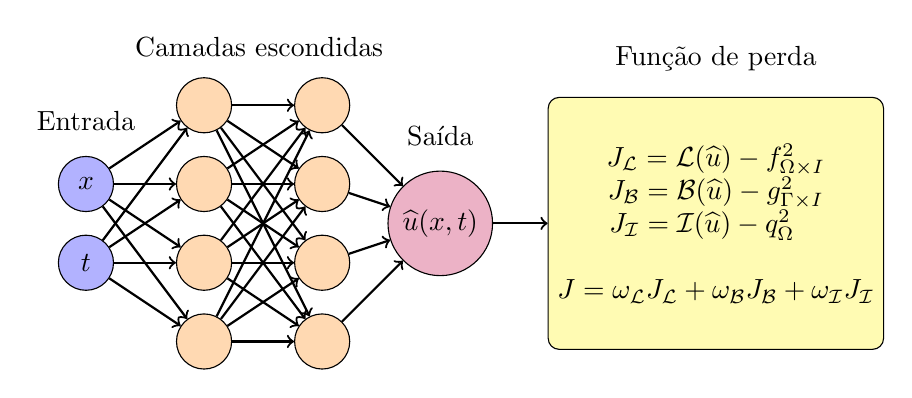
\begin{tikzpicture}[
    neuron/.style={circle, draw, minimum size=0.7cm},
    input/.style={neuron, fill=blue!30},
    hidden/.style={neuron, fill=orange!30},
    output/.style={neuron, fill=purple!30},
    physnode/.style={rectangle, draw, rounded corners, fill=orange!30, minimum width=1.5cm, minimum height=1.8cm},
    lossnode/.style={rectangle, draw, rounded corners, fill=yellow!30, minimum width=2cm, minimum height=3.2cm, align=center},
    every edge/.style={draw, ->, thick}
]

\node[input] (I-1) at (0, 2) {$x$};
\node[input] (I-2) at (0, 1) {$t$};

\node[hidden] (H1-1) at (1.5, 3) {};
\node[hidden] (H1-2) at (1.5, 2) {};
\node[hidden] (H1-3) at (1.5, 1) {};
\node[hidden] (H1-4) at (1.5, 0) {};

\node[hidden] (H2-1) at (3, 3) {};
\node[hidden] (H2-2) at (3, 2) {};
\node[hidden] (H2-3) at (3, 1) {};
\node[hidden] (H2-4) at (3, 0) {};

\node[output] (O-1) at (4.5, 1.5) {$\widehat{u}(x,t)$};

% Connections
\foreach \i in {1,2}
    \foreach \j in {1,...,4}
        \path (I-\i) edge (H1-\j);

\foreach \i in {1,...,4}
    \foreach \j in {1,...,4}
        \path (H1-\i) edge (H2-\j);

\foreach \j in {1,...,4}
    \path (H2-\j) edge (O-1);

\node[lossnode] (TotalLoss) at (8, 1.5) {
$J_{\mathcal{L}} = \lVert \mathcal{L}(\widehat{u}) - f \rVert^{2}_{\Omega \times I}$
\\
$J_{\mathcal{B}} = \lVert \mathcal{B}(\widehat{u}) - g \rVert^{2}_{\Gamma \times I}$
\\
$J_{\mathcal{I}} = \lVert \mathcal{I}(\widehat{u}) - q \rVert^{2}_{\Omega} \quad$
\\
\\
$J = \omega_{\mathcal{L}} J_{\mathcal{L}} + \omega_{\mathcal{B}} J_{\mathcal{B}} + \omega_{\mathcal{I}} J_{\mathcal{I}}$
};

\path (O-1) edge (TotalLoss);

% Labels
\node[above=0.2cm] at (I-1.north) {Entrada};
\node[above=0.2cm] at (2.2, 3.3) {Camadas escondidas};
\node[above=0.2cm] at (O-1.north) {Saída};
\node[above=0.2cm] at (TotalLoss.north) {Função de perda};

\end{tikzpicture}
\caption{Representação gráfica das PINNs. Fonte: elaborada pelos autores.}
\label{fig:pinn-representacao-grafica}
\end{figure}

\subsection{Pontos de Colocação}

Pontos de colocação são um conceito importante para as PINNs, sendo análogos
a criação da malha do \textit{MEF}. Entretanto, diferente do \textit{MEF}, 
não há um critério método bem definido para a obtenção destes pontos. 
Os pontos de colocação podem ser entendidos como uma discretização do domínio
de uma equação diferencial. O único critério que deve ser atendido é o uso
de pontos nas condições de fronteira e iniciais do problema.
Por esta perspectiva, os pontos de colocação podem ser entendidos como uma 
amostra do domínio na qual a rede neural será treinada. 
Por este motivo, muitas técnicas de amostragem multidimensional são 
aplicadas às PINNs para definir os pontos de colocação, pode-se citar como 
exemplo o hipercubo latino.   

\subsection{Formulação para Problemas Inversos}

A formulação para as PINNs apresentada até então foca na resolução de problemas
diretos. Em \cite{raissi-etal:19} é apresentada uma extensão para a mesma que 
também soluciona problemas inversos. Solucionar um problema inverso consiste em,
dado um conjunto de dados representados pela $\mathcal{L}_{\text{dados}}$,
encontrar um conjunto de parâmetros $\boldsymbol{\lambda}$ que minimaniza a
$\mathcal{L}_{\text{total}}$.
A equação \ref{eq:loss-total} pode então ser reescrita como,

\begin{eqnarray}\label{eq:loss-total-problema-inverso} 
    \mathcal{L}_{\text{total}}(\boldsymbol{\theta}, \boldsymbol{\lambda}) 
    = \omega_{\text{física}} \mathcal{L}_{\text{física}}(\boldsymbol{\theta}, \boldsymbol{\lambda}) 
    + \omega_{\text{dados}} \,\mathcal{L}_{\text{dados}}(\boldsymbol{\theta})
\end{eqnarray}

O problema de minimização descrito em \ref{eq:otimizacao-parametros} passa 
então a ser encontrar o conjunto $\boldsymbol{\theta}^*$ de parâmetros da rede,
como também o conjunto $\boldsymbol{\lambda}^*$
que minimiza a função \ref{eq:loss-total-problema-inverso}, 

\begin{equation}\label{eq:otimizacao-parametros-problema-inverso}
   (\boldsymbol{\theta}^*, \boldsymbol{\lambda}^*) 
   = \arg \min_{\boldsymbol{\theta}, \boldsymbol{\lambda}} \mathcal{L}_{\text{total}}(\boldsymbol{\theta}, \boldsymbol{\lambda}), 
\end{equation}

Vale salientar que a rede ao encontrar os conjuntos $\boldsymbol{\theta}^*$
e $\boldsymbol{\lambda}^*$, a rede neral está solucionando tanto o problema
direto (aproximar uma função que satisfaça as equações diferencias), quanto o 
problema inverso (encontrar $\boldsymbol{\lambda}^*$). 

\subsection{Arquiteturas Alternativas}

A definição de PINNs como uma rede neural com informação física não se aplica
apenas a redes \textit{feedfoward}, qualquer arquitetura de redes neurais
que incorpora as equações que descrevem os dados em que rede está sendo treinada, 
pode ser considerada uma rede neural informada pela física, uma PINN.

Desde a publicação do artigo seminal em 2019, uma série de arquiteturas 
alternativas foram propostas utilizando a ideia das PINNs como princípio.
Em \cite{shi-etal:24-convnet} é proposto uma arquitetura de rede convolucional
em que uma única camada convolucional é empregada. Nos testes realizados pelos
autores, a rede neural proposta apresentou uma convergência melhor do que uma 
PINN convecional para problemas de difusão com diferentes frequências. 

Em \cite{pang-etal:2019-fPINNs} é proposto uma arquitetura de redes neurais 
informadas pela física em que usa derivadas fracionárias na função de perda.
O modelo proposto, chamado de \textit{fPINNs}, é capaz de solucionar problemas 
clássicos como a equação de \textit{Burgers} utilizando derivadas parciais. 
O resultados são equiparáveis ao MEF.

Em \cite{sirignano-spiliopoulos:2018-deepgalerkin} é proposto o 
\textit{DeepGalerkin}, um método sem malhas para a solução de equações
diferencias de alta dimensionalidade que combina o método de Galerkin com
redes neurais. 

Baseado nas \textit{KANs} (\textit{Kolmogorov-Arnold Neural Networks})
\cite{liu-etal:2025-kans}, redes neurais baseadas no teorema de representação 
universal de Kolmogorov-Arnold utilizando, foram propostas em as 
\textit{PIKANs} (\textit{Physically Informed Kolmogorov-Arnold Neural Networks})
que combinando as funcões de ativação baseadas em \textit{b-splines} das
\textit{KANs} com a técnica de regressão simbólica para encontrar uma 
representação analítica das soluções encontradas pela rede neural.

\section{Modelos Compartimentais}

A utilização de equações diferencias para modelar fenõmenos físicos data desde do 
século XVIII. Modelos Compartimentais nada mais são do que modelos epidemiológicos
utilizados no estudo de doenças contagiosas que separam a população em grupos.
O fluxo entre esses grupos, chamados de compartimentos, é modelo por operações
de diferenciação.

\subsection{O modelo SIR}

Apresentado no trabalho seminal de \cite{kermack-mcKendrick:1927}, 
o modelo \textit{SIR} é definido pelo conjunto de equações \ref{eq:SIR-1}, 
\ref{eq:SIR-2} e \ref{eq:SIR-3}.

\begin{eqnarray}\label{eq:sir}
   \frac{dS(t)}{dt} &=& \frac{-\beta S(t)}{N} I(t),  \quad t > t_0, \label{eq:SIR-1}\\
   \frac{dI(t)}{dt} &=& \frac{\beta S(t)}{N} I(t) - \gamma I(t), \quad t > t_0, \label{eq:SIR-2}\\
   \frac{dR(t)}{dt} &=& \gamma I(t),  \quad t > t_0, \label{eq:SIR-3}
\end{eqnarray}

Estas três equações formam um sistema de equações diferencias de fácil interpretação.
A primeira equação modela a iteração entre pessoas infectadas e pessoas suscetíveis,
o parâmetro $\beta$, a taxa de infecção, diz quantos destes encontros resultaram 
em novos casos da doença. 
A terceira equação modela a recuperação de individuos ao
longo do tempo, o parâmetro $\gamma$ é taxa de individuos que se recuperam por 
unidade de tempo, sendo que a recuperação pode ser a cura da doença ou o falecimento
do individuo, já que o \textit{SIR} não distinguir os dois casos. 
A segunda equação é a soma do primeira e da terceira equação, mas com seus sinais
trocados. Ela modela o fluxo de indivíduos que entram e saem do compartimento
de infectados.  

Por se tratar de um sistema de equações diferencias ordinárias com três equações,
são necessárias três condições iniciais para se obter um problema de valor
inicial.

\begin{eqnarray}
   S(0) &=& S_0 \label{eq:SIR-S0}\\
   I(0) &=& I_0 \label{eq:SIR-I0}\\
   R(0) &=& R_0 \label{eq:SIR-R0}
\end{eqnarray}

Como o modelo não inclui mortes naturais ou por outras causas que não a doença
que está sendo modelada, nem o nascimento de pessoas na população estuda, assume-se
que a soma dos três comparimentos para qualquer tempo $t$ é igual ao total 
$N$ da popuiação,

\begin{equation}
   S(t) + I(t) + R(t) = N,  \quad t > t_0, \label{eq:SIR-4}
\end{equation}

O modelo pode ser entendido com um grafo em que os individuas fluem de um 
compartimento para outro a uma taxa $\beta$ e $\gamma$. 
A figura \ref{fig:sir-grafo} representa o \textit{SIR} por esta perspectiva.

\begin{figure}
\centering
\begin{tikzpicture}[
    node distance=2.5cm,
    box/.style={rectangle, minimum width=2cm, minimum height=1.5cm, 
                draw=black, thick, align=center, rounded corners=5pt,
                font=\large\bfseries},
    arrow/.style={-Stealth, thick, line width=1.2pt},
    label/.style={midway, sloped, font=\small}
]

    % Define nodes
    \node[box, fill=blue!20] (S) {Susceptible \\ S(t)};
    \node[box, fill=red!20, right=of S] (I) {Infected \\ I(t)};
    \node[box, fill=green!20, right=of I] (R) {Recovered \\ R(t)};

    % Transitions
    \draw (S) edge[->] node[label,above] {$\beta$} (I);
    \draw (I) edge[->] node[label,above] {$\gamma$} (R);

\end{tikzpicture}
\caption{Grafo para o \textit{SIR}. Fonte: elaborada pelos autores.}
\label{fig:sir-grafo}
\end{figure}

Certas definições são necessárias neste ponto para se compreender os modelos compartimentais. 
Em modelos epidemiológicos, incidência é o fluxo de novos casos por unidade de tempo,
enquanto que a prevalência é a quantidade de casos na população num instante $t$.
No caso do \textit{SIR}, estes conceitos são representados respectivamente pelo
termo $\frac{-\beta S(t)}{N}$ e pela equação $I(t)$. 

O número de reprodução básico $R_0$ é defido como a relação entre os parametros
$\beta$ e $\gamma$. Ele é de particular interesse para o estudo da propagação
de uma doença, pois se $R_0 > 1$, significa que a dispersão da doença
ainda está em curso e o número de infectados tende a aumentar. 
Se $R_0 < 1$, significa que a dispersão já atigiu seu pico e o número de individuos
infectados tender a diminuir. Se $R_0 = 1$ a doença está em equilíbrio e o número 
de infectados tender a se manter o mesmo.

\begin{equation}\label{eq:numero-reproducao-basico}
    R_0 = \frac{\beta}{\gamma}
\end{equation}

Um valor relacionado ao número de reprodução básico $R_0$, é o número de reprodução
efetivo $R_e$. Enquanto que o número de reprodução básico $R_0$ é utilizado para
medir o dispersão de uma doença no início de uma pandemia. 
Seu valor é obtido pela multiplicação de $R_0$ por $S$ num instante $t$.

\begin{equation}\label{eq:numero-reproducao-efetivo}
    R_e = R_0 S(t)
\end{equation}

O limite $\mathcal{T}$ define o valor máximo de indivíduos que estarão contaminados
no pico da pandemia. Este limite é importante para tomadores de decisão e governos
para entender os efeitos sobre os serviços de saúde pública.

\begin{equation}
    \mathcal{T} = \frac{\gamma}{\beta}N = \frac{N}{R_0}
\end{equation}

A figura \ref{fig:exemplo-sir} mostra um exemplo do \textit{SIR} com $\beta=0.8$
e $\gamma=0.1$ e as três curvas características desse modelo.

\begin{figure}[htpb]
\centering
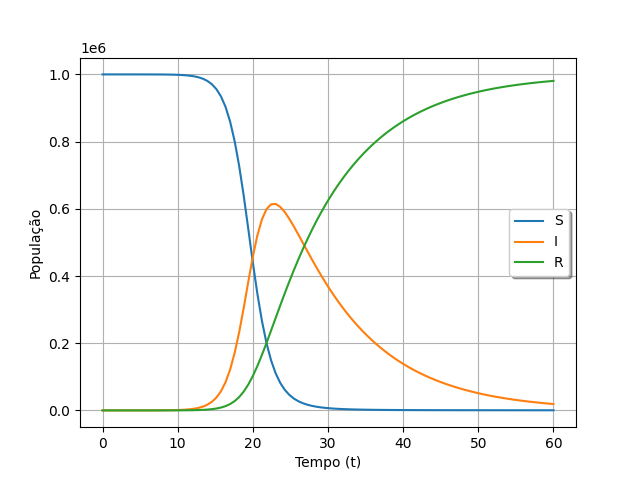
\includegraphics[width=0.6\textwidth]{figuras/sir-example-beta0.8-gamma0.1.png}
\caption{Exemplo do SIR com $\beta=0.8$ e $\gamma=0.1$.}
\label{fig:exemplo-sir}
\end{figure}

\subsection{Pontos de equilíbrio}

Os modelos compartimentais possuem dois pontos de equilíbrio chamados de 
ponto de equilíbrio livre de doenças e ponto de equilíbrio endemico. 
O primeiro ponto é atingido quando não há mais indivíduos infectados na população,
ou seja, nos ponto em que $I$ é igual a zero. O ponto de equilíbrio endêmico
é atigindo justamente quando o número de novos casos é compensado pelo número
de indivíduos que se recuperam.

\subsection{Adicionando Compartimentos}

Baseados no modelo \textit{SIR}, foram propostos outros modelos com mais 
compartimentos como o \textit{SEIRD} \cite{giles:77-sird} que inclui um 
compartimento para individuos que foram expostos a doença, mas 
ainda não manifestaram sintomas. 
Outro exemplo é o \textit{SIRV} \cite{schlickeiser-kroger:21-sirv} 
que inclui um compartimento para vacinados.
Outro exemplo de modelo recente é o \textit{SVIHRD} \cite{nelson-etal:24-japao}
que inclui compartimentos para hospitalizados e vacinados.

\section{Matriz de nova geração}

Uma forma de se calcular o número de reprodução básico $R_0$ é a aplicar a técnica
de matriz de nova geração\dots

\section{Problemas Inversos}

Problemas inversos são mal-postos\dots

Identificabilidade de um modelo\dots

PINNs para smalldata\dots

\section{Aplicação de PINNs com Modelos Compartimentais}

Com a pandemia de COVID-19 no fim de 2019, renovou-se o interesse em modelos
epidemiológicos compartimentais. As PINNs, que haviam acabado de ser propostas,
foram encaradas como uma ferramenta nova que poderia ser utiizada junto com 
a grande quantidade de dados que estavam sendo gerados. 
Nesta seção são apresentados alguns trabalhos que aplicaram PINNs para solucionar
problemas em epidemiologia. São destacados novos modelos compartimentais, 
modificações feitas nos modelos clássicos, e aplicações inovadoras das PINNs.  

Em \cite{ouyoussef-etal:24-subcompartimentos} é apresentada uma variação
do \textit{SIR} em os compartimentos de suscetíveis e infectados 
são divididos em dois subgrupos. Há também um subgrupo de indivíduos 
vacinados \textit{V}, que assume constante ao longo do tempo do tempo, 
sendo que apenas uma porcentagem $\xi$ está totalmente imunizada.
Os autores não estavam interessados na taxa de recuperação, logo ela é assumida
como constante e a terceira equação do sistema \textit{SIR} é removida. 
A PINN passa a ter que aproximar as quatro curvas de interesse do modelo 
($S_1$, $S_2$, $I_1$, $I_2$), 
além de descobrir, as quatro taxas 
($\beta_{11}$, $\beta_{12}$, $\beta_{21}$ e $\beta_{22}$) de infecção
A aplicação destes subgrupos varia conforme a modelagem, 
pode se dividir a população por grupos de risco, por exemplo.
O modelo passaria a capturar as iterações entre estes subgrupos.
São feitos testes apenas com dados sintéticos. 

Outro exemplo utilizando subgrupos dentro dos compartimentos pode ser encontrado
em \cite{arulandu-etal:23-vacinacao}. Mas os autores vão além, ao utilizar 
o modelo de meta-populações de \cite{jacquez:1988-modelagam-hiv-matriz} que 
divide a população em $n$ subcompartimentos, transformando o parâmetro $\beta$ 
numa matriz $n \times n$. Através de simplificações algébricas, é proposto uma 
variação do \textit{SIR} com $3n$ equações e $3n + 3$ parâmetros.
Os autores então empregam este modelo junto com uma PINN para estimar o número 
de reprodução efetivo $R_i$ para cada população $i$, sendo $i \in [1,...,n]$. 
Este valor é então usado para ajudar na criação de um plano de vacinação que 
priorize populações mais vulneráveis, ou seja, aquelas em que $R_i$ é maior.
São realizados testes com a famosa base de dados sobre a dispersão de influenza
numa escola londrina.  

Modelos compartimentais utilizam sistemas de ODEs para modelar a evolução
de uma pandemia, considerando apenas o tempo como variável independente e 
ignorando a dimensão espacial.
Em \cite{bertaglia-etal:22-sir-reacao-difusao} é feita uma modificação do 
modelo \textit{SIR}, criando o \textit{SIR} hiperbólico. 
A modificação consiste em inser uma dimensão espacial e transformar o PVI
num problema de reação-difusão, numa EDP hiperbólica em função da dimensão espacial $x$
e temporal $t$. A função de perda da rede é modificada, mas tomando cuidado
para garantir que rede satisfaça a propriedades de convergência assintótica.
São realizados testes envolvendo problemas diretos e inversos para averiguar
a efetividade do modelo.

O uso de PINNs com modelos com mais compartimentos é explorado em \cite{nelson-etal:24-japao}.
O autores propõem o já mencionado \textit{SVIHRD}, um modelo que inclui 
compartimentos para vacinados (\textit{V}), hospitalizados (\textit{H}), 
e separa o compartimento de recuperados em entre os que se curaram e as 
fatalidades (\textit{D}).
O compartimento de hospitalizados é usado para medir a ocupação dos serviços de
saúde pública.
O modelo ainda inclui uma taxa de nascimentos para os 
suscetíveis e uma taxa de mortes naturais para todos os outros compartimentos.
É demonstrada a estabilidade do modelo e são feitos testes com dados da pandemia 
de COVID-19 no Japão.

Em \cite{han-etal:24-prim-artigo-alemanha} há um outro exemplo de aplicação de
PINNs com modelos comportimentais e parâmetros que variam no tempo. Os autores
aplicaram o modelo \textit{SAIRD} para gerar dados sintéticos para 
o treinamento de uma PINN. Uma vez validado o modelo, ele é utilizado para se
ajustar aos dados de COVID-19 da Alemanha. É feito um estudo sobre o
parâmetro $\omega_{\text{dados}}$ para diferentes valores e seus efeitos na 
convergência da rede e valores obtidos para os parâmetros do problema inverso. 

Um dos primeiros usos de PINNs com parâmetros variando no tempo é proposto em 
\cite{long-etal:21-L2}. Os autores aplicam uma PINN com o modelo \textit{SIRD}
para estimar a taxa de transmissão da COVID-19 em três cidades americanas
ao longo de março de 2020 a outrubro de 2020. Uma vez calculada a estimativa da 
taxa de transmissão ao longo do tempo, o número de reprodução básico é calculado
para o mesmo período. 
Os parâmetros estimados são alimentados numa \textit{Long Short Term Memory} 
(LSTM) para prever o número de infectados no mês seguinte, outubro. 

Em \cite{shamsara-etal:25-omicron} é apresentado uma aplicação de PINNs
junto ao modelo \textit{SVIHRD} com parâmetros variando no tempo. 
Os autores introduzem uma técnica para ajustar o peso $\omega_{\text{dados}}$ 
ao longo do treinamento da rede. O modelo é então aplicado
para ajustar a dados de COVID-19 dos países Itália, França e Alemanha. 
Uma vez estimada a taxa de transmissão da doença, ela é correlacionada com O
surgimento de variantes do vírus que causa a COVID-19.

Outra extensão feita nos modelos clássicos é proposta em \cite{nguyen-etal:22-raissi-seirp}.
Os autores modificam o \textit{SEIR} ao adicionar um compartimento $P$ para 
modelar a concentração de patogêneos em ambientes fechados, e a possibilidade
de contaminação pela doença através da interação não apenas com o contato com
individuos contaminados, mas também com a iteração com pantogêneos presentes no
ambiente. Os autores deduzem os pontos de equilíbrio do modelo e 
realizam testes com PINNs nos dados de influenza de um colègio
privado londrino.     

Um exemplo com modelos de ordem fracionária é apresentado em 
\cite{li-etal:25-ordem-fracionaria}. Os autores utilizam uma versão do 
\textit{SEIHDR} (\textit{Susceptible-Exposed-Invected-Hospitalized-Deacesed-Recovered}) 
com derivadas fracionárias de Caputo e parâmetros variando no tempo.
São feitas análises dos pontos de estabilidade do modelo, e o número de reprodução
básico é calculado utilizando matrizes de próxima geração. 
As PINNs são usadas para ajustar o modelo aos dados de COVID-19 do Canadá.

Em \cite{heldmann-etal:23-biobjective-opt} é aplicado o modelo \textit{SVIHRD}
com uma função de custo multi-objetivo ao tratar a $\mathcal{L}_{\text{física}}$
e a $\mathcal{L}_{\text{dados}}$ como duas funções objetivos distintas.
A função de perda da rede é composta por uma aproximação da curva Pareto entre 
as duas funções objetivos.
Outra inovação do artigo, é estimar alguns parâmetros utilizando o métedo de 
diferenças finitas alternativo. 
As PINNs são aplicadas para os dados de COVID-19 da Alemanha. São feitos ajustes
aos dados para estimar os parâmetros de transmissão e previsões de curto tempo.  

A combinação de modelos compartimentais com PINNs podem ser utilizados para 
outros fins que não apenas estimar a taxa de transmissão da doença.
Em \cite{ghosh-etal:23-subnotificacao} é apresentado uma variação do \textit{SEIR}
com níveis de imunidade dependentes do tempo e do número de doses de vacinas 
ministradas, o modelo também considera a eficácia da vacina. 
Estas adições ao \textit{SEIR} são modeladas na forma de parâmetros extras que 
podem mover indivíduos do compartimento de recuperados para o compartimento de
suscetíveis.
O modelo é aplicado junto a PINNs para estimar o nível de subnotificação de 
infectados e mortes não atribuídas a COVID-19 na China após o fim da política 
de COVID zero.

Outro exemplo que combina PINNs com métodos já consolidados na literatura
pode ser encontrado em \cite{millevoi-etal:24-split-join-pinns}.
Os autores propõem uma chamada "abordagem separada" (\textit{split approach}),
a ideia principal é separar o treinamento da rede em duas fases. Na primeira 
fase, o compartimento de infectados é aproximado utilizando uma rede neural
que se ajusta aos dados. Na segunda fase, a saída desta rede é então utilizada
junto a uma PINN para para estimar o número de suscetíveis e a taxa de transmissão
$\beta$ do modelo \textit{SIR}. A vantagem desta abordagem em comparação com a
abordagem tradicional, ou "conjunta" (\text{joint approach}) é simplificar a 
função de perda da rede neural ao simplificar as equações do modelo \textit{SIR}
que são usadas na função de perda, fazendo com que a PINN tenha uma curva a menos 
para se ajustar, melhorando a convergência da mesma. Os autores
testam a abordagem proposta com dados sintéticos e para dados de COVID-19 da Itália,
além de testes com lacunas nos dados para testar a resiliência da proposta. 

Outro exemplo  \cite{shaier-etal:22-dinns}

Em \cite{ogueda-oliva:23-colombia-duas-cidades} é feita uma modificação no
modelo \textit{SIRD} para modelar o descolocamento de pessoas duas 
cidades colombianas de Bogotá e Medellín. A incorporação deste movimento 
é feita através de uma matriz de transporte e o resultado é um modelo \textit{SIRD}
com duas populações distintas e, por consequência, dois compartimentos para cada
compartimento original ($S_1$, $S_2$, $I_1$, $I_2$, ...), assim como parâmetros 
duplicados ($\beta_1$, $\beta_2$, $\gamma_1$, $\gamma_2$, ...). O modelo é utilizado
para se ajustar aos dados de COVID-19 da Colômbia de 2021.

\cite{ning-etal:23-pinns-paralelas} são usadas PINNs paralelas...

Mais  \cite{hu-etal:22-identificabilidade}

Um exemplo utilizando redes neurais recorrentes pode ser encontrado 
em \cite{rodriguez-etal:2022-einns}

% No artigo original, são utilizados \textit{Multi-layer Perceptrons} (MLPs)
% como arquitetura das redes, mas há propostas com utilizando outras arquiteturas.
% Uma proposta utilizando redes neurais convolucionais pode ser encontrada em 
% \cite{shi-etal:24-convnet}. Uma proposta utilizando PINNs combinado com 
% métodos Bayesianos pode ser encontrada em \cite{yang:21-bpinns}, esta 
% abordagem é particulamente interessante para problemas inversos, ao transformar
% a estimativa dos parâmetros numa distribuição, no lugar de um valor fixo.
